% Created 2014-10-09 木 17:51
\documentclass[t]{beamer}
\usepackage{zxjatype}
\usepackage[ipa]{zxjafont}
\setbeamertemplate{navigation symbols}{}
\hypersetup{colorlinks,linkcolor=,urlcolor=gray}
\AtBeginSection[]
{
  \begin{frame}<beamer>{Outline}
  \tableofcontents[currentsection,currentsubsection]
  \end{frame}
}
\setbeamertemplate{navigation symbols}{}
\usepackage[utf8]{inputenc}
\usepackage[T1]{fontenc}
\usepackage{fixltx2e}
\usepackage{graphicx}
\usepackage{longtable}
\usepackage{float}
\usepackage{wrapfig}
\usepackage{rotating}
\usepackage[normalem]{ulem}
\usepackage{amsmath}
\usepackage{textcomp}
\usepackage{marvosym}
\usepackage{wasysym}
\usepackage{amssymb}
\usepackage{hyperref}
\tolerance=1000
\usepackage{minted}
\usetheme{Madrid}
\author{産業技術大学院大学 \linebreak 中鉢 欣秀}
\date{2014-10-09}
\title{Scrumと要求工学}
\hypersetup{
  pdfkeywords={},
  pdfsubject={},
  pdfcreator={Emacs 24.3.1 (Org mode 8.2.6)}}
\begin{document}

\maketitle


\section{enPiTについて}
\label{sec-1}
\begin{frame}[label=sec-1-1]{enPiTについて}
\begin{itemize}
\item enPiT(エンピット)は最先端の情報技術を実践的に活用することができる
人材育成を目指しています。
\item クラウドコンピューティング、セキュリティ、組込みシステム、
ビジネスアプリケーションの4つの分野において、
大学と産業界による全国的なネットワークを形成し、
実践的な情報教育の普及・推進を図ります。
\end{itemize}
\end{frame}

\begin{frame}[label=sec-1-2]{AIITのenPiTにおけるアジャイル開発}
\begin{itemize}
\item 事前学習
\begin{itemize}
\item アジャイル開発の方法論
\item アジャイル開発で利用するツール
\end{itemize}
\item Project Based Learning
\begin{itemize}
\item Scrumによりプロジェクトを実施
\item 毎週1回のレビュー
\item 期間は11週間
\end{itemize}
\end{itemize}
\end{frame}

\section{アジャイル開発における要求の取り扱い}
\label{sec-2}
\begin{frame}[label=sec-2-1]{企画・アイディアの段階}
\begin{block}{エレベータピッチ}
\begin{itemize}
\item 忙しくて時間をとってもらえないエグゼクティブや重役に対して、
こちらの無力を伝えるプレゼンテーションを
重役室までのエレベーターの中というごく短時間の中で行なうこと
\end{itemize}
\end{block}
\begin{block}{リーンキャンバス}
\begin{itemize}
\item ビジネスのアイディアを一目瞭然にする(詳細は省略)
\end{itemize}
\end{block}
\end{frame}

\begin{frame}[label=sec-2-2]{Scrumにおける要求}
\begin{block}{Product owner (PO)}
\begin{itemize}
\item 製品の所有者
\item POの定義は様々
\begin{itemize}
\item 製品の仕様に責任を持つ人
\item 製品を投入するマーケットをよく知っている人
\item スティーブジョブスのこと
\end{itemize}
\end{itemize}
\end{block}
\begin{block}{Product backlog (PB)}
\begin{itemize}
\item 「ユーザーストーリー」等の集合
\begin{itemize}
\item 製品のビジョンを実現するために必要な機能
\end{itemize}
\item POが優先順位をつける
\item POはPBを活発に更新する
\end{itemize}
\end{block}
\end{frame}

\begin{frame}[label=sec-2-3]{ユーザストーリーのルール(INVEST)}
\begin{itemize}
\item Independent(独立している)
\item Negotiable(交渉可能)
\item Valuable(価値がある)
\item Estimable(見積り可能)
\item Sized right / Small(適切な大きさ)
\item Testable(テスト可能)
\end{itemize}
\end{frame}

\begin{frame}[label=sec-2-4]{「PBの項目はReadyであること」}
\begin{itemize}
\item 下記のような例は満たされない
\begin{itemize}
\item そもそもなんのためにそのPB項目があるのか分からない
\item PB項目の内容が曖昧または抽象的すぎて、作るべきものが分からない。または人によって著しく成果物のイメージが異なる
\item PB項目に受け入れ条件がないため、何ができたらそのバックログ項目が完了になるのか分からない
\item PB項目の受け入れ条件が抽象的もしくは測定困難(クールな画面とか応答が速いとか)
\item 同様にPB項目のデモの仕方がわからない
\item PB項目が大きすぎて、1つの項目に含まれる作業が膨大になってしまう。それ故抜け漏れが大量に発生する
\item PB項目の他への依存度が高すぎて、具体的な作業内容や作業順序のイメージがつかない
\end{itemize}
\end{itemize}
\end{frame}

\section{Scrumと要求工学}
\label{sec-3}
\begin{frame}[label=sec-3-1]{要求工学との関連}
\begin{itemize}
\item Scrumにおける「要求の獲得」
\begin{itemize}
\item POと開発者が話し合い,PBを成長させる
\end{itemize}
\item Scrumにおける「要求の記述」
\begin{itemize}
\item Product backlogを用いる
\end{itemize}
\end{itemize}
\end{frame}

\begin{frame}[label=sec-3-2]{Scrumで忘れ去られていること}
\begin{itemize}
\item より形式的な記述やモデル化
\begin{itemize}
\item PBはユーザの言葉だとして,
SBに「モデル化」や「仕様化」の作業が入るはず
\end{itemize}
\item 非機能要求
\begin{itemize}
\item だれがどう定義するのか
\end{itemize}
\item Product/Sprint Backlogの品質
\begin{itemize}
\item Backlogの品質や望ましい書き方は?
\item そのための体系的な方法は?
\begin{itemize}
\item 制限言語?
\end{itemize}
\end{itemize}
\end{itemize}
\end{frame}

\section{レビューを中心としたスタイル}
\label{sec-4}
\begin{frame}[label=sec-4-1]{ハッカソン「Demo or die」}
\begin{itemize}
\item 考え方
\begin{itemize}
\item 毎回必ず動くソフトウエアのデモをして見せる
\item どんなプレゼン資料よりも正しく現状が共有できる
\end{itemize}
\item スプリントごとのデモ
\begin{itemize}
\item 最新の製品が常にレビューできるようになっていること
\end{itemize}
\end{itemize}
\end{frame}

\begin{frame}[label=sec-4-2]{ツールの連携とレビューのサイクル}
\begin{figure}[htb]
\centering
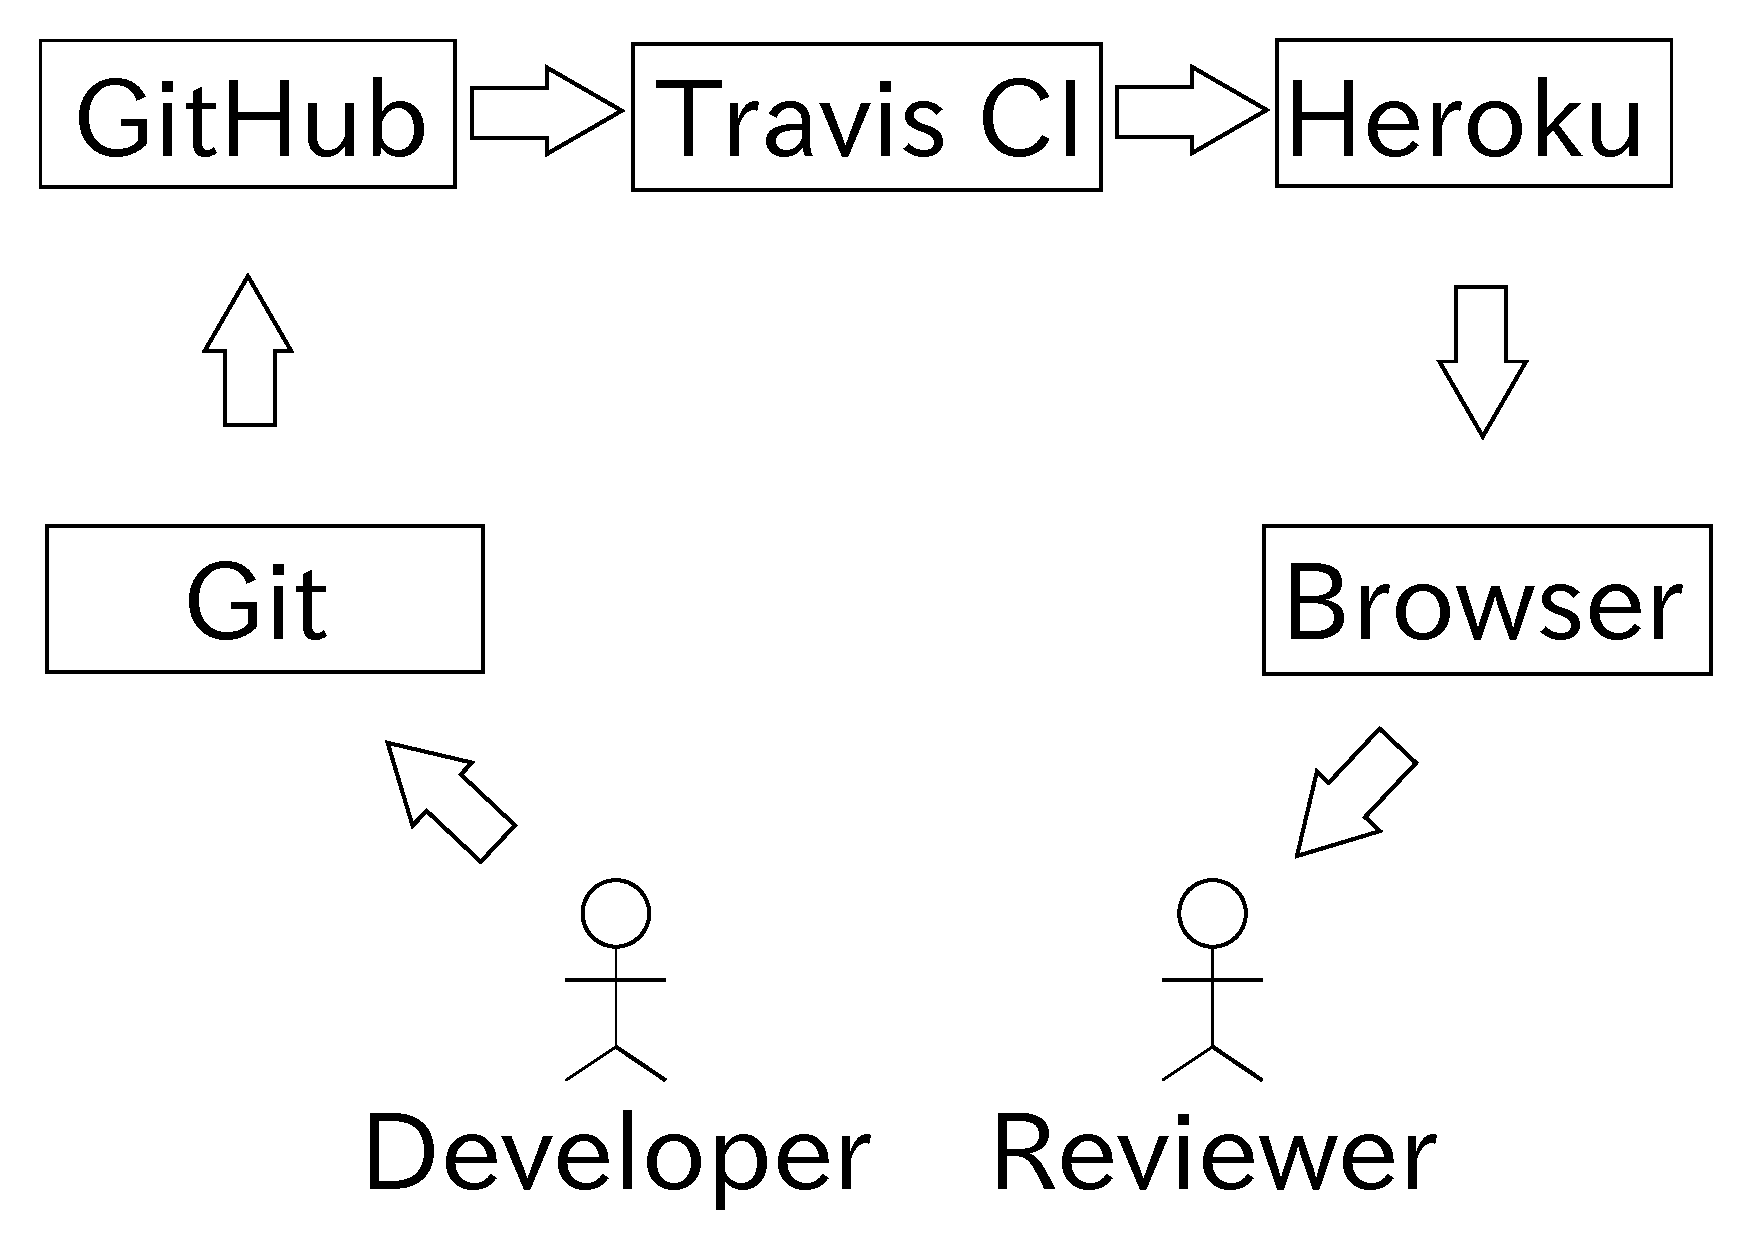
\includegraphics[width=.75\linewidth]{./tools.pdf}
\caption{\label{fig:tools}Tools used in enPiT Program.}
\end{figure}
\end{frame}

\begin{frame}[label=sec-4-3]{enPiTのPBLの様子}
\begin{itemize}
\item いつでもデモができるようになっている
\item \href{https://github.com/ychubachi/enpit/wiki/\%E5\%88\%86\%E6\%95\%A3PBL\%EF\%BC\%882014\%EF\%BC\%89}{分散PBL(2014) · ychubachi/enpit Wiki}
\end{itemize}
\end{frame}

\section{参考文献}
\label{sec-5}
\begin{frame}[label=sec-5-1]{参考文献}
\begin{itemize}
\item \href{http://kray.jp/blog/attractive-product-backlog/}{魅力的なプロダクトバックログで開発を楽しく! | KRAY Inc}
\item \href{http://www.ryuzee.com/contents/blog/5024}{\{Scrum\}プロダクトバックログ項目の明確化の必要性 | Ryuzee.com}
\item \href{http://master-consultant.jp/\%E3\%82\%A8\%E3\%83\%AC\%E3\%83\%99\%E3\%83\%BC\%E3\%82\%BF\%E3\%83\%BC\%E3\%83\%94\%E3\%83\%83\%E3\%83\%81\%E3\%81\%AE\%E4\%BD\%9C\%E3\%82\%8A\%E6\%96\%B9/}{一瞬で見込みクライアントのハートをつかむエレベーターピッチの作り方 | コンサル大学 トップ4%のコンサルタントになる!}
\item \href{http://www.slideshare.net/studytech/ss-23454300}{リーンキャンバスとは}
\end{itemize}
\end{frame}
% Emacs 24.3.1 (Org mode 8.2.6)
\end{document}